\section{Experiment}
%\begin{figure}[t]
%	\centering
%	%\fbox{\rule{0pt}{2in} \rule{0.9\linewidth}{0pt}}
%	\includegraphics[width=0.8\linewidth]{experiment.png}
%	
%	\caption{Assessing the Similarity Between Network Activation and Brain Activation.}
%	\label{fig:fig3}
%\end{figure}
%\label{sec:experiment}

\subsection{Benchmarks} \label{sec:Dataset}

\hspace{1pc}All evaluations are conducted on the Carla~\cite{Dosovitskiy:2017}. 
We assess our methods using the nocrash \cite{codevilla2019exploring} and leaderBoard datasets. 
Each benchmark specifies its own training scenes and weather conditions for data collection, and evaluates the agent's performance in new towns and weather settings. 
The nocrash dataset focuses on generalization from Town01, a European town with one-lane roads and T-junctions, to Town02, a smaller variant of Town01 with different textures. 
In contrast, the LeaderBoard presents a more challenging generalization task across six maps with various traffic scenarios, including freeways, US-style junctions, roundabouts, stop signs, and lane changes. 
Following the nocrash dataset~\cite{codevilla2019exploring}, we test generalization from four training weather types to two new weather types, though only two training weather types are evaluated to save computational resources. 
The nocrash benchmark includes three traffic density levels (empty, regular, and dense), defining the number of pedestrians and vehicles per map. 
We focus on the nocrash-dense setting and introduce a new level, nocrash-busy, which lies between regular and dense traffic to avoid congestion typical in dense traffic settings. 
For the offline LeaderBoard, traffic density is adjusted to match the busy traffic setting. 


% CILv2
As with recent top-performing methods \cite{Hu:2022}, for on-board data collection in CARLA, we use the \emph{teacher} expert driver from \cite{Zhang:2021}, referred to as Roach RL.
This method, based on reinforcement learning and trained with privileged information, exhibits more realistic and diverse behavior compared to the default (handcrafted) expert driver in CARLA. 
It is important to note that in real-world experiments, we would use human drivers as experts.
We adopt the default settings from \cite{Zhang:2021}, which means, similar to the student driver in \cite{Zhang:2021} (RIM) and in \cite{Hu:2022} (MILE), the ego-vehicle is the 2017 Lincoln model available in CARLA.
Each of the three forward-facing cameras on the ego-vehicle has a resolution of $W\times H=300\times300$ pixels, with a horizontal field of view (HFOV) of $60^{\circ}$.
The cameras are arranged without overlap, collectively covering a total HFOV of $180^{\circ}$, centered along the main axis of the ego-vehicle.


Using the expert driver, ego-vehicle, and on-board cameras, we collect data for progressively more complex experiments.
First, we gather a dataset from CARLA's Town01, a small town that only allows single-lane driving, meaning lane change maneuvers are not possible.  
% 中午、傍晚、大雨的中午、潮湿的中午
Specifically, we collect 15 hours of data at 10 fps (approximately 540K frames per camera view) under four training weather conditions: ClearNoon, ClearSunset, HardRainNoon, and WetNoon. 
% 测试:Town02 细雨的傍晚、潮湿的傍晚
For generalization testing, we use CARLA's Town02, evaluating the agent under SoftRainSunset and WetSunset weather conditions. 
Next, we collect a dataset across multiple CARLA towns to capture more complex driving scenarios, such as multi-lane driving, highway entrances and exits, and passing through crossroads. 
To maintain consistency with the setup in \cite{Hu:2022}, we reserve Town05 for testing, and gather 25 hours of data at 10 fps from Town01 to Town06 (5 hours per town, totaling approximately 900K frames per camera). 
Both training and testing weather conditions remain the same for Town01 and Town02.



\subsection{Implementation Details}

\hspace{1pc}To optimize Eq. (\ref{eq:loss}), we use the Adam optimizer \cite{Kingma:2015} with an initial learning rate of $10^{-4}$ and weight decay of $0.01$. 
Training is performed for 80 epochs on a single NVIDIA A6000 GPU, with a batch size of 120.
The learning rate is reduced by half at epochs 30, 50, and 65.


% Cornet详细信息
In ventral stream, after the input is processed by V2$_\text{COR}$ once, the resulting output is passed back into V2$_\text{COR}$ and treated as a new input, while the original input is discarded.
V2$_\text{COR}$ and IT$_\text{COR}$ are repeated twice, and V4$_\text{COR}$ is repeated four times, as this configuration yielded the best model performance based on our evaluation scores.
Similar to ResNet, each convolution (except the first $ \times $ convolution) is followed by batch normalization and a ReLU activation.
Batch normalization is not shared across time steps.
The current definition of the ventral pathway does not include across-area bypass or feedback connections, and retinal and LGN processing are not explicitly modeled.


% 驾驶评估的3个不同数据集(不包含实验结果)
\subsection{Driving Evaluation}
\label{sec:Metrics}
\hspace{1pc}The performance of the BID agent is limited by the performance of the expert it is imitating. 
If the expert performs poorly, the agent that mimics it will also show suboptimal results. 
The BID model is designed to closely follow the visual information processing system of the human brain, both structurally and functionally. 
When optimized, the model’s output closely matches the expert’s performance, as evaluated by similarity metrics.


We conduct experiments on small single-lane town (Sec.~\ref{sec:small_town_results}) following the nocrash dataset~\cite{Zhang:2021,Hu:2022}, and on multiple towns (Sec.~\ref{sec:small_town_results}) based on the offline CARLA leaderboard benchmark~\cite{Zhang:2021,Hu:2022}. 


\subsubsection{Nocrash Evaluation}\label{nocrash_metrics}

\hspace{1pc}The benchmark consists of three tasks with increasing levels of difficulty: \emph{Empty}, \emph{Regular}, and \emph{Dense}, based on the number of dynamic objects in the scene ({\ie}, pedestrians and vehicles). 
In Town02, the numbers of dynamic objects are specified as:
\begin{itemize}
	\item \emph{Empty}: 0 pedestrians and 0 vehicles;
	\item \emph{Regular}: 50 pedestrians and 15 vehicles;
	\item \emph{Dense}: 150 pedestrians and 70 vehicles
\end{itemize}
% 默认的配置会导致拥堵死锁
In the \emph{Dense} case, the default traffic density in nocrash often results in congestion and deadlocks at intersections~\cite{Zhang:2021}. 
To address this, we adopt the \emph{Busy} case redefined in~\cite{Zhang:2021}, reducing the number of pedestrians from 150 to 70. 
Each task consist of 25 goal-directed episodes under two new weather conditions.
An episode is terminated and counted as a failure if a collision occurs. 
For other infractions, the driving score is penalized according to the rule specified in nocrash. 


% 度量标准的说明
The primary metric for comparing driving models is the success rate (\emph{SR}), which represents the percentage of episodes that are successfully completed. 
% 严格的成功率
For a more detailed comparison, we also provide the strict success rate (\emph{S.SR}),
% traffic infraction:交通违法行为
which measures the percentage of successful episodes under a zero tolerance policy for any traffic infractions, such as failing to stop at a red light or deviating from planned route.
% T.L:在红灯时不停的次数
Additionally, we include other infraction metrics.
\emph{T.L}: the number of times the vehicle fails to stop at a red traffic light.
% 和其他车辆碰撞的次数
\emph{C.V}: The number of collisions with other vehicles.
% R.Dev:当高层命令没有很好地执行,路线偏差的次数
\emph{R.Dev}: The number of route deviations, where the high-level command is not proerly executed.
% O.L:考虑了自主车辆驶出车道的情况(例如,在对面车道或人行道上)
\emph{O.L}: The number of times the ego-vehicle drives out of its lane ({\eg}, into the opposite lane or onto the sidewalk).
% C.L:与城镇布局发生碰撞的次数
\emph{C.L} is the number of collisions with the town layout. 
All infraction values are normalized per kilometer driven.


\subsubsection{Offline Leaderboard Metrics.}\label{lb_metrics}
\hspace{1pc}To align our evaluation with CARLA leaderboard\cite{Hu:2022}, we use the offline CARLA Leaderboard metrics for multiple towns. 
% Avg.DS 平均驾驶分数、平均路线完成
The key metrics are the average driving score (\emph{Avg.DS}) and the average route completion (\emph{Avg.RC}). 
\emph{Avg.DS} penalizes driving performance based on the criteria defined in the CARLA Leaderboard, 
% Avg.RC:自车辆能够行驶至目标的平均距离。
while \emph{Avg.RC} measures the average distance the ego-vehicles is able to travel toward the goal.


% 高层导航命令
\subsubsection{High-level Navigation Commands} 
\hspace{1pc}As in CILRS \cite{Codevilla:2019}, during training, we use simple navigation commands such as ``continue in the lane" or ``go-straight/turn-left/turn-right" when reaching an intersection.
However, in more complex towns, after crossing an intersection, the ego-vehicle may legally enter any of the multiple available lanes. 
Since this information is avaiable through the global navigation system, if the ego-vehicle deviates from the pre-planned trajectory by entering a different lane, a corrective command is issued, such as ``move to left lane" or ``move to right lane" as soon as possible. 
This corrective mechanism is only applied during testing. 
An example of this process is shown in Figure~\ref{fig:command_ambiguous}.

% 各种环境下的场景说明
% Roach_carla0913_fps10_dense_normalcamera_NoCrash_3cam/RouteScenario_0000/rgb_central001215.png
\begin{figure}[t]
	\centering
	\includegraphics[width=1.0\linewidth]{fig/dataset_examples.pdf}
	\caption{Top: When the ego-vehicle is driving on the road, even though the triffic light is green, the vehicle in front has stopped, but the ego-vehicle still brakes.
	Bottom: When the vehicle is moving and encounters a traffic jam in front, it will automaitcally brake and stop.
	The brake command in the figure is displayed in \textcolor{red}{red}.}
	\label{fig:command_ambiguous}
\end{figure}


% 三种不同场景的性能
\begin{table*}
	\caption{Town02 nocrash results.
		RIM refers to Roach IL and the Expert refers to Roach RL~\cite{Zhang:2021}. 
		All models are tested on CARLA 0.9.13. 
		Mean values and standard deviations are computed from three runs with different seeds. 
		For metrics denoted with $\uparrow$, higher values indicate better performance, while for those marked with $\downarrow$, lower values are preferable.}
	\centering
	\resizebox{0.95\linewidth}{!}{
		\begin{tabular}{@{}lccc|ccc|ccc@{}}
			\hline
			& \multicolumn{3}{c}{Empty} & \multicolumn{3}{c}{Regular} & \multicolumn{3}{c}{Busy}  \\
			
			& \textbf{$\uparrow$ SR(\%)} & \textbf{$\uparrow$ S.SR(\%)} & $\downarrow$ T.L  & \textbf{$\uparrow$ SR(\%)} & \textbf{$\uparrow$ S.SR(\%)} & $\downarrow$ T.L & \textbf{$\uparrow$ SR(\%)} & \textbf{$\uparrow$ S.SR(\%)} & $\downarrow$ C.V \\
			\hline
			
			RIM\cite{Zhang:2021}  & $100\pm0.0$ & $85\pm1.2$ & $66\pm5.0$ & $97\pm2.3$ & $86\pm7.2$ & $66\pm54$ & $81\pm5.0$& $68\pm7.2$ & $63\pm52.7$\\
			CIL++\cite{xiao2023scaling} & $100\pm0.0$ & $100\pm0.0$ & $0\pm0.0$  & $99\pm2.3$ & $97\pm3.1$ & $7\pm7.9$ & $83\pm7.6$ & $77\pm7.6$ & $45\pm21.5$ \\
			Our BID & $100\pm0.0$ & $100\pm0.0$ & $0\pm0.0$  & $99\pm2.3$ & $97\pm3.1$ & $7\pm7.9$ & $83\pm7.6$ & $77\pm7.6$ & $45\pm21.5$ \\
			\hline
			Expert & $100\pm0.0$ & $100\pm0.0$ & $0\pm0.0$ & $100\pm0.0$ & $97\pm0.0$ & $13\pm4.6$ & $84\pm2.0$ & $82\pm2.0$ & $37\pm14.1$ \\
			\hline 
		\end{tabular}
	}
	\label{tab:T2_NC_results}
\end{table*}


\begin{table*}
	\caption{Town05 results based on CARLA's offline metrics. 
		All models are tested on CARLA 0.9.13. 
		Mean values and standard deviations are computed from three runs with different random seeds.
		For metrics marked with $\uparrow$, higher values indicate better performance, while for those marked with $\downarrow$, lower values are preferred.}
	\centering
	\resizebox{0.88\linewidth}{!}{
		\begin{tabular}{@{}lccccccccccccccccccccc@{}}
			\hline
			%   & SR(\%) 
			%   & S.SR(\%) 
			& \textbf{$\uparrow$ Avg.RC(\%)} & \textbf{$\uparrow$ Avg.DS }
			& $\downarrow$ C.V & $\downarrow$ C.L & $\downarrow$ T.L & $\downarrow$ O.L & $\downarrow$ R.Dev 
			\\
			\hline
			RIM\cite{Zhang:2021}  & $92\pm3.1$ & $51\pm7.9$ 
			& $7.5\pm1.3$ & $4.3\pm1.6$ & $26.0\pm8.9$ & $5.4\pm2.7$ & $3.0\pm3.2$ & \\
			MILE~\cite{Hu:2022}
			& $98\pm2.2$ & $73\pm2.9$ 
			& $6.0\pm3.7$ & $0.0\pm0.0$ & $3.6\pm3.8$ & $3.5\pm1.5$ & $0.0\pm0.0$ \\   
			CIL++\cite{xiao2023scaling} 
			& $98\pm1.7$ & $68\pm2.7$ 
			& $6.0\pm0.5$ & $3.8\pm0.7$ & $5.8\pm5.1$ & $6.1\pm2.2$ & $9.4\pm3.6$ \\
			Our BID 
			& $98\pm1.7$ & $68\pm2.7$ 
			& $6.0\pm0.5$ & $3.8\pm0.7$ & $5.8\pm5.1$ & $6.1\pm2.2$ & $9.4\pm3.6$ \\
			\hline
			Expert 
			& $99\pm0.8$ & $89\pm1.7$ 
			& $3.2\pm1.1$ & $0.0\pm0.0$ & $1.3\pm0.4$ & $0.0\pm0.0$ & $0.0\pm0.0$ \\
			\hline
		\end{tabular}
	}
	\label{tab:T5_results}
\end{table*}


\subsection{Experimental Results}
\label{sec:Results}
% 基于模型的模仿学习
\hspace{1pc}We compare BID with three state-of-the-art, vision-based eend-to-end autonomous driving models: the Roach IL model (here RIM) \cite{Zhang:2021}, MILE \cite{Hu:2022} and CIL++\cite{xiao2023scaling}. 
It is important to note that although BID uses data generated by the Roach RL model, training a BID model does not require human-labeled sensor data. 
In this case, the Roach RL model acts as a human driver during data acquisition. 
In contrast, training a RIM model requires supervision from the Roach RL expert, who is trained with privileged information, while MILE is trained using semantic Bird’s Eye View (BeV) data for supervision.


\subsubsection{Small Single-lane Towns} \label{sec:small_town_results}

\hspace{1pc}We first conduct initial experiments using CARLA's Town01 and Town02, along with the nocrash evaluations(Sec.~\ref{nocrash_metrics}). 
Town01 is used for training, while Town02 is reserved for testing (Sec.~\ref{sec:Dataset}). 
MILE provides a model trained on multiple CARLA towns, but no model is available that is specifically trained on Town01 alone. 
On the other hand, RIM has models trained on both Town01 and multiple towns. To ensure a fair comparison, we only use RIM’s model trained on Town01. 
In Table~\ref{tab:T2_NC_results}, we present the success rate (SR) and strict success rate (S.SR) for the different traffic densities (Empty, Regular, Busy). 
For a more focused evaluation, we report T.L (traffic light violations) for the Empty and Regular cases, and C.V (collisions with vehicles) only for the Busy case. 
It is important to note that scenarios with fewer or no dynamic obstacles are more effective for evaluating the ego-vehicle's reaction to red traffic lights, while collisions are more appropriately assessed in scenarios with higher traffic density and more dynamic objects.


In general, BID achieves the best results across all tasks. 
In the Empty case, BID significantly outperforms RIM in avoiding traffic light infractions, contributing to a higher S.SR. 
This conclusion holds true in the Regular case as well. 
In the Busy case, BID comes close to matching the expert’s performance, again outperforming RIM in terms of S.SR and resulting in fewer collisions with vehicles. 
For the expert, failure cases in Busy scenarios are primarily due to traffic deadlocks, which cause a timeout in route completion. 
Despite this, the expert's performance can still be considered a valid upper bound.


\subsubsection{Multi-town Generalization}\label{sec:multi_towns_result}
\hspace{1pc}In this section, we evaluate the performance of BID in more complex scenarios provided by CARLA’s multiple towns. 
As outlined in Sec.~\ref{sec:Dataset}, for a fair comparison, we align the training and testing settings with those used in MILE~\cite{Hu:2022}, and use CARLA’s offline Leaderboard metrics (Sec.~\ref{lb_metrics}). 
The results for all models trained on multi-town data are presented in Table~\ref{tab:T5_results}. 
RIM performs the worst among the three models, incurring more infractions and resulting in a significantly lower Avg.DS. 
BID achieves an Avg.RC of 98\%, which is comparable to MILE. 
However, in terms of Avg.DS, MILE scores the highest at 73\%, while BID achieves 68\%. 
We attribute this difference to the fact that MILE rarely drives outside the pre-planned lane, as it is provided with the route map as input. 
In contrast, BID does not use an explicit route map and instead relies solely on high-level navigation commands.

% 不同迭代时的消融实验
% CILv2_multiview\network\models\architectures\CIL_multiview\evaluator.py
\begin{figure*}[t]
	\centering
	\includegraphics[width=0.99\textwidth]{fig/driving_scores.pdf}
	\vspace{-1ex}
	\caption{\textbf{Driving performance and training progress of BID.} 
		All BID agents are evaluated in LBCRoutes after 30 peoch.
		Top figure: The ground truth and model prediction for steering angles are shown in green and blue, respectively.
		Bottom figure: The errors in training progress are displayed every 5 epochs, including the mean absolute error (MAE) for steering and acceleration.
		Results are reported as the mean over 5 evaluation seeds, while other metrics are evaluated with single seed. 
		The offline Leaderboard benchmark is used for evaluation.}
	\vspace{-1.5ex}
	\label{fig:score_eu_lb_tt_tn}
\end{figure*}


% 在密集场景中的消融实验
% table:sucess_rate_nc_dense
\begin{table}
	\caption{\textbf{Success rate of camera-based end-to-end imitation learning agents on nocrash-dense.}
		The mean and standard deviation are computed over 5 seeds. 
		% 数据聚合方法:DAGGER:试图在学习策略诱导的状态分布下收集专家演示
		Our models are from DAGGER iteration 5. 
		For DA-RB, ``+" indicates triangular perturbations have been added to the off-policy dataset, ``(E)" denotes an ensemble of all iterations.}
	\setlength{\tabcolsep}{6.67pt}
	\centering
	\begin{tabular}{lccccc}
		\hline
		Success Rate \% $\uparrow$
		&  NCd-tt & NCd-tn  & NCd-nt & NCd-nn  \\ 
		\hline
		% \cmidrule(lr){1-1}\cmidrule(lr){2-5}
		SAM \cite{zhao2021sam} (0.8.4) & 
		$54 \pm 3$ & $47 \pm 5$ & $29 \pm 3$ & $29 \pm 2$ \\
		LBC \cite{chen2020learning} (0.9.6) & 
		$71 \pm 5$ & $63 \pm 3$ & $51 \pm 3$ & $39 \pm 6$ \\
		LSD \cite{ohn2020learning} (0.8.4) & 
		N/A & N/A & $30 \pm 4$ & $32 \pm 3$ \\
		DA-RB\textsuperscript{+}(E) \cite{prakash2020exploring} & 
		$66 \pm 5$ & $56 \pm 1$ & $36 \pm 3$ & $35 \pm 2$ \\
		DA-RB\textsuperscript{+} \cite{prakash2020exploring} (0.8.4)  & 
		$62 \pm 1$ & $60 \pm 1$ & $34 \pm 2$ & $25 \pm 1$ \\
		Our baseline, $\mathcal{L}$ & 
		$\mathbf{88} \pm 4$ & $29 \pm 3$ & $32 \pm 11$ & $28 \pm 4$ \\
		Our improved, $\mathcal{L}_\text{D} $ & 
		$\mathbf{88} \pm 4$ & $29 \pm 3$ & $32 \pm 11$ & $28 \pm 4$ \\
		Our best, $\mathcal{L}_\text{D}+\mathcal{L}_\text{N}$ & 
		$86 \pm 5$ & $\mathbf{82} \pm 2$ & $\mathbf{78} \pm 5$ & $\mathbf{78} \pm 0$ \\
		\hline
	\end{tabular}
	\vspace{-1ex}
	\label{table:sucess_rate_nc_dense}
	\vspace{-2ex}
\end{table}

\begin{table*}
	\caption{\textbf{Driving performance and infraction analysis of BID agents on nocrash-busy, new town \& new weather.} 
		The mean and standard deviation are reported over 5 evaluation seeds.}
	\setlength{\tabcolsep}{7.4pt}
	\centering
	\begin{tabular}{lccccccccc} 
		\hline
		& \begin{tabular}{@{}c@{}}Success \\ rate \end{tabular} 
		& \begin{tabular}{@{}c@{}}Driving \\ score \end{tabular} 
		& \begin{tabular}{@{}c@{}}Route \\ compl. \end{tabular} 
		& \begin{tabular}{@{}c@{}}Infrac. \\ penalty \end{tabular} 
		& \begin{tabular}{@{}c@{}}Collision \\ others \end{tabular} 
		& \begin{tabular}{@{}c@{}}Collision \\ pedestrian \end{tabular} 
		& \begin{tabular}{@{}c@{}}Collision \\ vehicle \end{tabular}  
		& \begin{tabular}{@{}c@{}}Red light \\ infraction \end{tabular}  
		& \begin{tabular}{@{}c@{}}Agent \\ blocked \end{tabular}  \\
		\hline
		% \cmidrule(lr){1-1}\cmidrule(lr){2-5}\cmidrule(lr){6-10}
		iter 5
		& \%, $\uparrow$
		& \%, $\uparrow$
		& \%, $\uparrow$
		& \%, $\uparrow$
		& \#/Km, $\downarrow$
		& \#/Km, $\downarrow$
		& \#/Km, $\downarrow$
		& \#/Km, $\downarrow$
		& \#/Km, $\downarrow$
		\\
		\hline
		%\cmidrule(lr){1-1}\cmidrule(lr){2-5}\cmidrule(lr){6-10}
		$\mathcal{L}_\mathrm{b}$
		& $32 \pm 5$ & $42 \pm 3$ & $61 \pm 5$ & $76 \pm 4$ 
		& $0.53 \pm 0.55$ & $\mathbf{0}\pm0$ & $0.63 \pm 0.50$ & $3.33 \pm 0.58$ & $19.4\pm 14.4$ \\
		$\mathcal{L}_\text{D}$
		& $58\pm6$ & $65\pm3$ & $85\pm2$ & $76\pm1$ 
		& $2.06\pm1.28$ & $\mathbf{0}\pm0$ & $1.37\pm1.10$ & $1.5\pm0.2$ & $2.83\pm1.46$ \\
		$\mathcal{L}_\text{N}$
		& $75\pm2$ & $78\pm0$ & $90\pm2$ & $85\pm1$ 
		& $0.51\pm0.25$ & $\mathbf{0}\pm0$ & $0.52\pm0.17$ & $0.69\pm0.06$ & $3.36\pm0.21$ \\
		$\mathcal{L}_\text{D}+\mathcal{L}_\text{N}$
		& $\mathbf{88} \pm 5$ & $\mathbf{89} \pm 3$ & $\mathbf{97} \pm 0$ & $\mathbf{90} \pm 3$ 
		& $\mathbf{0.07} \pm 0.04$ & $0.01 \pm 0.01$ & $\mathbf{0.22} \pm 0.07$ & $\mathbf{0.62} \pm 0.22$ & $\mathbf{0.83} \pm 0.03$ \\
		\hline
		%\cmidrule(lr){1-1}\cmidrule(lr){2-5}\cmidrule(lr){6-10}
		$\mathcal{L}_\text{BID}$
		& $96 \pm 2$ & $96 \pm 3$ & $99 \pm 0$ & $97 \pm 2$ 
		& $0 \pm 0$ & $0.12 \pm 0.08$ & $0.03 \pm 0.06$ & $0.14 \pm 0.18$ & $0 \pm 0$ \\
		Expert
		& $91 \pm 1$ & $78 \pm 2$ & $97 \pm 1$ & $81 \pm 2$ 
		& $0 \pm 0$ & $0 \pm 0$ & $0.19 \pm 0.07$ & $1.92 \pm 0.22$ & $0.17 \pm 0.09$\\
		\hline
	\end{tabular}
	\vspace{-1ex}
	\vspace{-2.5ex}
	\label{table:infraction}
\end{table*}


% 可视化注意力
\subsubsection{Visualizing BID's Attention}
\label{sec:Visualization}
\hspace{1pc}We are interested in understanding which parts of the image BID focuses on during decision-making. 
To achieve this, we use Grad-CAM~\cite{Selvaraju:2017}, where gradients flow from the action space to the final convolutional layer of the ResNet backbone. 
This process generates a heatmap that highlights the image regions most important for action prediction. 
However, since BID addresses a regression task, its output can take both positive and negative values, while Grad-CAM is originally designed for image classification tasks, where outputs are always positive. 
To adapt Grad-CAM for our case, we cannot simply focus on the positive gradients of the feature map. 
Instead, the computation is split into two cases based on the sign of the output value. 
Negative gradients are used to compute the feature map weights when the acceleration or steering angle is negative, and positive gradients are used when the output is positive.


% _results\_results\CILv2\CILv2_3cam_single_lane\Eval\Valid_gradCAM_Roach_LBCRoutes_3cam_valid\30\-1\85.jpg
Fig.~\ref{fig:attention_ped_greed} illustrates the activation map at an intersection. 
Three regions of the image are highly activated: the traffic light on the right, the crossing pedestrians in the center, and the lane shoulder on the left. 
This suggests that BID demonstrates a proper understanding of the scene and a clear connection between its observations and actions. 
Specifically, BID decides to brake because of the pedestrians, even though the traffic light is green and the navigation command is to turn left. 
This indicates that BID appropriately prioritizes the presence of pedestrians over the traffic signal and navigation command.


% 验证集的1350帧,激活图的第45张
\begin{figure}[ht!]
	\centering
	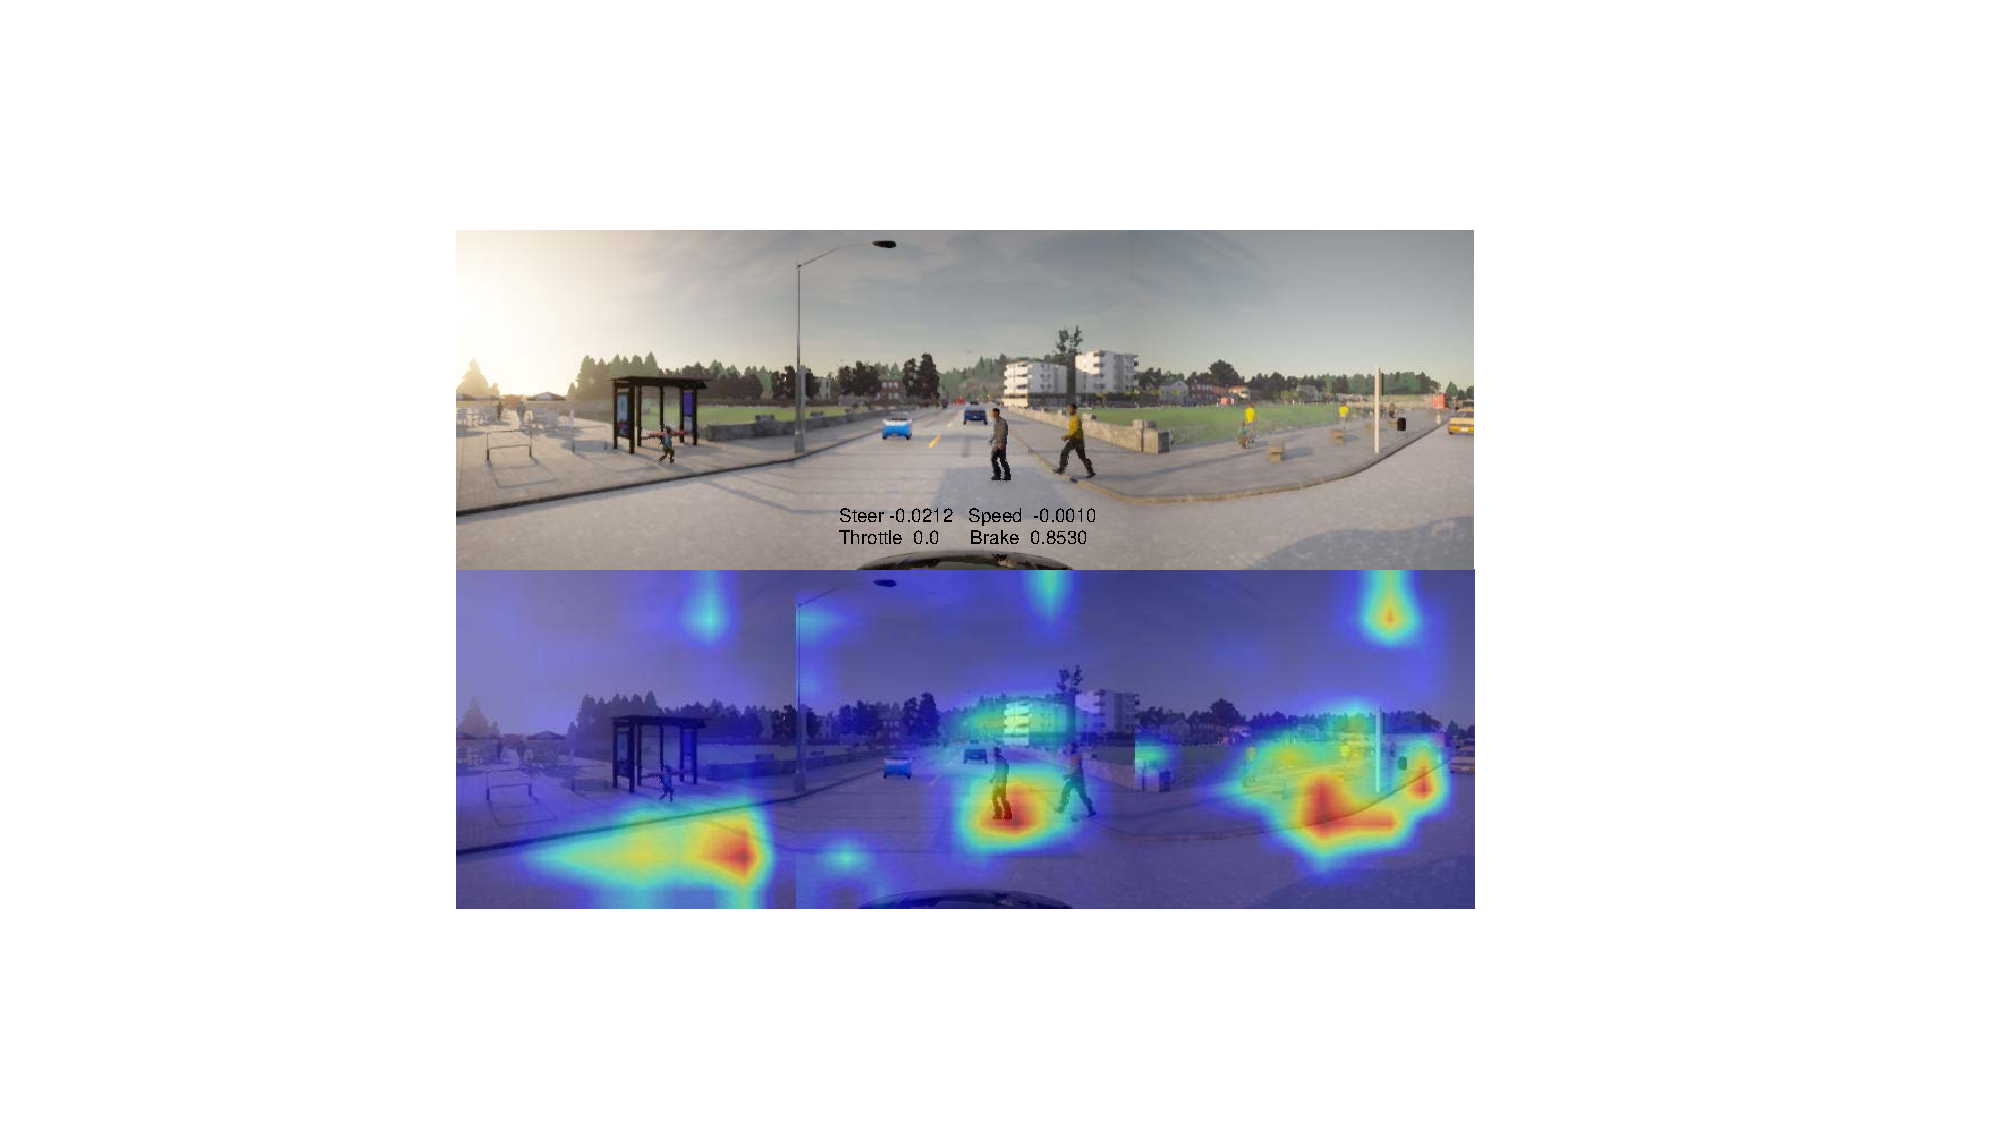
\includegraphics[width=\linewidth]{fig/attention_ped_greed.pdf}
	\caption{Activation maps of BID at an intersection in Town02 show three highly activated image areas from driving viewpoints: 
		the lane shoulder in the right image, the crossing pedestrians in the center, and the driving area in the left image. 
		The causality between observation and action is demonstrated by a strong braking response (0.8530) due to the presence of pedestrians, despite the ``go-straight" command. 
		This highlights BID's ability to prioritize pedestrian safety over other factors in its decision-making process.}
	\label{fig:attention_ped_greed}
\end{figure}



% 消融实验:速度(包括背侧通路)、导航
\subsubsection{Ablation}

\hspace{1pc}The performance of an IL agent is inherently limited by the quality of the expert it imitates. 
If the expert's performance is poor, it is not meaningful to compare IL agents trained on that expert. 
This issue becomes apparent in the nocrash new town scenario with dense traffic, where autopilots typically perform poorly. 
To establish a high-performance upper bound and ensure a fair comparison, we training the BID (Fig.~\ref{fig:score_eu_lb_tt_tn}) and conduct ablation studies (Table~\ref{table:infraction}) under the busy traffic setting, allowing our Autopilot to achieve a driving score of 78\% and a success rate of 91\%. 
For a more meaningful comparison with state-of-the-art models, the best-performing configuration from the ablation studies is also evaluated on nocrash with dense traffic, as shown in Table~\ref{table:sucess_rate_nc_dense}.


% 说明消融的各个指标?
% L_N 导航信号
% L_D 背侧流信号
Fig.~\ref{fig:score_eu_lb_tt_tn} shows the driving scores of experts and IL agents at each DAGGER iteration on nocrash and offline LeaderBoard with busy traffic.
The baseline $\mathcal{L}$ represents our implementation of the baseline BID trained by expert. 
According to the LeaderBoard instructions, this additional navigation vector helps disambiguate situations where the semantics of left and right may be unclear due to the complexity of the map.
Given the improvements in our best-performing BID, it is expected that $\mathcal{L}_\text{D}$ and $\mathcal{L}_\text{D} + \mathcal{L}_\text{N}$ achieve higher success rates than those reported in Table~\ref{table:sucess_rate_nc_dense}.
The significant performance gap between the baseline and $\mathcal{L}_\text{D} + \mathcal{L}_\text{N}$, especially when generalizing to a new town and new weather, highlights the limitations of the baseline approach.


% 一步步添加后的效果
By incorporating the dorsal stream and speed embedding into the baseline $\mathcal{L}_\text{b}$, $\mathcal{L}_\text{D}$ outperforms $\mathcal{L}_\text{b}$ overall.
Additionally, learning from the action distribution allows $\mathcal{L}_\text{D}$ to generalize better than $\mathcal{L}_\text{b}$ on the nocrash dataset, but not on the offline LeaderBoard.
Feature matching only improves performance when $E_s$ is provided with the necessary information to produce accurate driving action.
In our case, $E_N$ contains navigational information since the desired route is given throught nagivation command.
For the LeaderBoard, navigational information is partially encoded in $E_N$, which includes the vector pointing to the next desired waypoint, leading to improved performance with the use of $E_N$.
To evaluate this idea, we utilize a integrated network architecture where the measurement vector $E_N$ is augmented with the navigation command encoded as a one-hot vector.
With feature matching applied to this architecture, $\mathcal{L}_\text{BID}$ achieves the best driving score among IL agents in the nocrash new town and weather generalization test, even outperforming the Autopilot.



%
Adding value supervision alongside feature matching accelerates the convergence of the DAGGER process, as demonstrated by $\mathcal{L}_\text{D} + \mathcal{L}_\text{N}$.
However, when feature matching is omitted, value supervision alone does not lead to superior performance with $\mathcal{L}_\text{D}$.
This suggests a potential synergy between feature matching and value estimation. 
Intuitively, the latent feature of Roach encodes the necessary information for value estimation, so mimicking this feature should assist in predicting the value. 
In turn, value estimation can help regularize feature matching, improving overall performance.


\subsubsection{Infraction and Performance Analysis}


\hspace{1pc}Table~\ref{table:infraction} presents a detailed performance and infraction analysis on the nocrash dataset with busy traffic in the new town and weather setting. 
Notably, the extremely high ``Agent blocked" rate in our baseline $\mathcal{L}_\text{A}(\text{a})$ is primarily caused by reflections from after-rain puddles. 
This issue is significantly reduced by imitating Roach, which drives more naturally, leading to a 23\% absolute improvement in the driving score for $\mathcal{L}_\text{D}$. 
This gain reflects the benefit of using a better expert, while keeping the same imitation learning approach. 
Further improvements are achieved with the addition of soft targets and latent feature supervision in $\mathcal{L}_\text{D}+\mathcal{L}_\text{N}$, resulting in another 30\% absolute increase in performance. 
By handling red lights more effectively, this BID agent achieves a driving score of 89\%, reaching expert-level performance with just camera image as input.





 